% Séquence 2 : Points et droites
\setseqtitle{Points et droites}
\chapter{Points et droites}
\label{chap:seq02}

% ======= Petits outils locaux (utilisables dans tout le chapitre) =======
% Pointillés pour les réponses (remplace \underline{\hspace{...}})
\newcommand{\trou}[1]{\makebox[#1]{\dotfill}}
% Styles TikZ (si déjà définis dans le préambule, ces lignes n'ont pas d'effet néfaste)
\tikzset{
	pt/.style   ={circle,fill=black,inner sep=1.2pt},
	lbl/.style  ={font=\footnotesize, inner sep=1pt},
	seg/.style  ={line width=0.9pt},
	dro/.style  ={line width=0.9pt},
	para/.style ={line width=0.9pt, dashed}
}

\begin{objectifsbox}
	\textbf{Vocabulaire et notations :} point, segment, demi-droite, droite, lectures [AB], (AB), [AB), AB.\\
	\textbf{Relations :} appartenance, alignement, droites sécantes/perpendiculaires/parallèles.\\
	\textbf{Méthodes :} tracer des parallèles et des perpendiculaires (règle + équerre).
\end{objectifsbox}

% =========================
\section*{1) Vocabulaire et notations}
\begin{itemize}
	\item Un point est un lieu dans le plan ; on le nomme par une \trou{5cm} majuscule.
	\item Une \trou{5cm} est une ligne définie par \trou{3cm} points distincts ; elle est \trou{3cm} (s'étend à l'infini).
	La droite passant par $A$ et $B$ se note : \trou{5cm}.
	\item Un \trou{3cm} est une portion de \trou{3cm} délimitée par deux \trou{3cm} appelés \trou{3cm}.
	On le note : \trou{3cm}.
	\item Une \trou{3cm} est une partie de \trou{2.2cm} qui commence en un \trou{3cm} donné et s'étend à l'infini.
	On la note par exemple : \trou{3cm}.
\end{itemize}

\textbf{Lecture :} $[AB]$ se lit << \trou{3cm} >> ; $(AB)$ se lit << \trou{3cm} >> ; $[AB)$ se lit << \trou{3cm} >> ;
$AB$ se lit << \trou{3cm} >> (ou << \trou{3cm} >>).

% --- Figure vocabulaire : droite, segment, demi-droite, longueur AB
\begin{figure}[h]
	\centering
	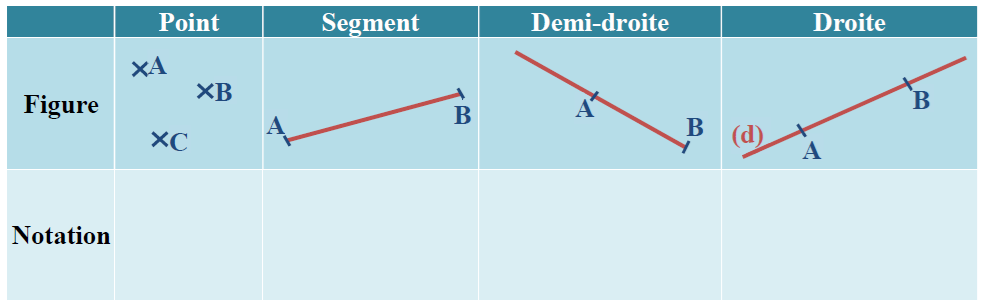
\includegraphics[width=1\linewidth]{../../../assets/images/6e/seq_02/points_segment_droites.png}
	\caption{Vocabulaire : $(AB)$ droite ; $[CD]$ segment ; $[EF)$ demi-droite ; $AB$ longueur.}
	\label{fig:vocab-points-droites}
\end{figure}

% =========================
\section*{2) Appartenance et alignement}
\begin{itemize}[label = \textbullet]
	\item $A$ \trou{1cm} $(d)$, $B$ \trou{1cm} $(d)$, $C$ \trou{1cm} $(d)$ ; $K$ \trou{1cm} $(d)$.
	\item Définition : Des points sont dits \textbf{alignés} s'ils \trou{6cm}.
\end{itemize}

% --- Figure appartenance et alignement
\begin{figure}[h]
	\centering
	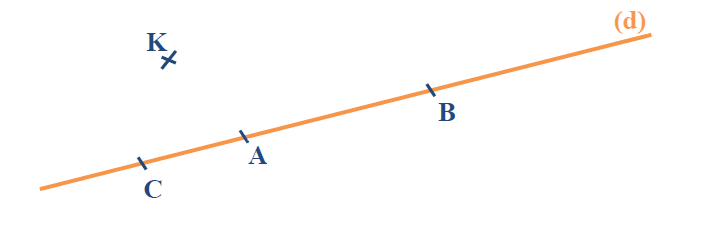
\includegraphics[width=1\linewidth]{../../../assets/images/6e/seq_02/pt_sur_dte.png}

	\label{fig:point-sur-droite}
\end{figure}

% =========================
\section*{3) Positions relatives des droites}
\begin{itemize}
	\item Deux droites sont \textbf{sécantes} si elles se coupent en \trou{1.2cm} point.
	\item Deux droites sont \textbf{perpendiculaires} si elles se coupent en formant un \trou{1.5cm} \trou{1.5cm}. On note : $(d)\perp(d')$.
	\item Deux droites sont \textbf{parallèles} si elles ne sont pas \trou{2.2cm}. On note : $(AB)//(EF)$.
\end{itemize}

\textbf{Lecture :} $(AB)//(EF)$ se lit << \trou{5cm} >> (ou << \trou{5cm} >>). \quad $(d)\perp(\Delta)$ se lit << \trou{5cm} >>.

% --- Figures sécantes / perpendiculaires / parallèles
\begin{figure}[h]
	\centering
	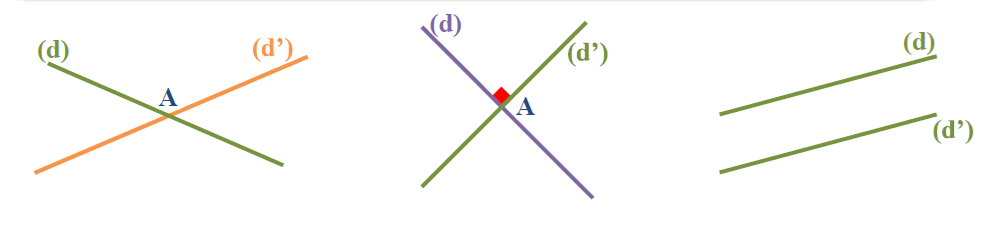
\includegraphics[width=1\linewidth]{../../../assets/images/6e/seq_02/position_relative.png}
	%\caption{Vocabulaire : $(AB)$ droite ; $[CD]$ segment ; $[EF)$ demi-droite ; $AB$ longueur.}
	\label{fig:Position relative de droites}
\end{figure}

% =========================
\section*{4) Tracer à la règle et à l'équerre}
\begin{itemize}
	\item Perpendiculaire à $(d)$ passant par $A$ : placer l'\trou{2.5cm} sur $(d)$, aligner le petit \trou{2.3cm}, faire un repère par $A$, tracer la droite \trou{2.3cm} à $(d)$.
	\item Parallèle à $(d)$ passant par $B$ : avec \trou{2.3cm} et équerre, faire glisser l'équerre en conservant le \trou{2.3cm} ; quand un côté passe par $B$, tracer la \trou{2.3cm} à $(d)$.
\end{itemize}

% --- Figures de construction : perpendiculaire en A, parallèle par B
\begin{figure}[h]
	\centering
	\begin{tikzpicture}[scale=1]
		% Perpendiculaire en A
		\begin{scope}[shift={(-4,0)}]
			\coordinate (A) at (-0.5,0.2);
			\coordinate (B) at (2,0);
			\draw[dro] (-2,0.15)--(2.2, -0.05); % (d)
			\node[lbl,below right] at (1.9,-0.05) {$(d)$};
			\node[pt] at (A) {}; \node[lbl,above] at (A) {$A$};
			% perpendiculaire
			\draw[dro] ($(A)!-1!(90:1)$) -- ($(A)!1!(90:1)$);
			\fill[gray!30] (A) -- ($(A)+(0.35,0)$) -- ($(A)+(0.35,0.35)$) -- ($(A)+(0,0.35)$) -- cycle;
			\node[lbl] at (-0.5,-0.7) {Perpendiculaire en $A$};
		\end{scope}
		
		% Parallèle par B
		\begin{scope}[shift={(3.5,0)}]
			\coordinate (P) at (-1.8,0.1);
			\coordinate (Q) at (1.8,-0.05);
			\draw[dro] (-2,0.1)--(2,-0.05); % (d)
			\node[lbl,below right] at (1.9,-0.08) {$(d)$};
			\coordinate (B) at (0.2,1.0);
			\node[pt] at (B) {}; \node[lbl,above] at (B) {$B$};
			% parallèle par B (même direction que (d))
			\draw[para] ($(B)+(-2,0.15)$)--($(B)+(2,0.0)$);
			\node[lbl] at (0.2,0.5) {Parallèle par $B$};
		\end{scope}
	\end{tikzpicture}
	\caption{Constructions : perpendiculaire en $A$ ; parallèle passant par $B$.}
	\label{fig:constructions}
\end{figure}

% =========================
\section*{5) Existence et unicité}
\begin{itemize}
	\item Par deux points distincts, il passe \trou{1.5cm} droite et une seule.
	\item Par un point donné $A$, il existe \trou{1.5cm} droite \trou{2cm} à $(d)$ ; elle est \trou{1.4cm}.
	\item Par un point donné $A$, il existe \trou{1.5cm} droite \trou{2cm} à $(d)$ ; elle est \trou{1.4cm}.
\end{itemize}

% =========================
\section*{6) Je m'entraîne}
\begin{itemize}
	\item Lecture : $[MN]$, $(RS)$, $[TU)$, $VU$.
	\item Notations : << La droite passant par $P$ et $Q$ >> ; << Le segment $KL$ >> ; << La demi-droite d'origine $H$ passant par $J$ >> ; << La longueur $AB$ >>.
	\item Complète : Si $A \in (BC)$ alors $A,B,C$ sont \trou{2cm}. Si $D \notin (EF)$ alors $D$ \trou{2cm} à la droite $(EF)$.
\end{itemize}
